\documentclass{extarticle}
\usepackage[utf8]{inputenc}
\usepackage{amsmath}
\usepackage{amssymb}
\usepackage{tikz}
\usepackage{fancyhdr}
\usepackage{geometry}

\geometry{letterpaper, margin=1in}
\pagestyle{fancy}
\fancyhf{}
\lhead{Complex Test Document}
\rhead{Page \thepage}

\title{Complex LaTeX Document}
\author{Test Author}
\date{\today}

\begin{document}

\maketitle

\section{Advanced Math}
Complex equation with multiple lines:
\begin{align}
    \int_{-\infty}^{\infty} e^{-x^2} dx &= \sqrt{\pi} \\
    \sum_{n=1}^{\infty} \frac{1}{n^2} &= \frac{\pi^2}{6} \\
    \lim_{x \to 0} \frac{\sin x}{x} &= 1
\end{align}

\section{TikZ Graphics}
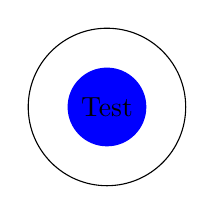
\begin{tikzpicture}
    \draw (0,0) circle (1cm);
    \fill[blue] (0,0) circle (0.5cm);
    \node at (0,0) {Test};
\end{tikzpicture}

\section{Tables}
\begin{table}[h]
    \centering
    \begin{tabular}{|c|c|c|}
        \hline
        A & B & C \\
        \hline
        1 & 2 & 3 \\
        4 & 5 & 6 \\
        \hline
    \end{tabular}
    \caption{Test Table}
\end{table}

\end{document}